% ======================================================================
% common-fontsize-de.tex
% Copyright (c) Markus Kohm, 2001-2022
%
% This file is part of the LaTeX2e KOMA-Script bundle.
%
% This work may be distributed and/or modified under the conditions of
% the LaTeX Project Public License, version 1.3c of the license.
% The latest version of this license is in
%   http://www.latex-project.org/lppl.txt
% and version 1.3c or later is part of all distributions of LaTeX 
% version 2005/12/01 or later and of this work.
%
% This work has the LPPL maintenance status "author-maintained".
%
% The Current Maintainer and author of this work is Markus Kohm.
%
% This work consists of all files listed in MANIFEST.md.
% ======================================================================
%
% Paragraphs that are common for several chapters of the KOMA-Script guide
% Maintained by Markus Kohm
%
% ======================================================================

\KOMAProvidesFile{common-fontsize-de.tex}
                 [$Date: 2022-10-06 14:30:20 +0200 (Do, 06. Okt 2022) $
                  KOMA-Script guide (common paragraphs: fontsize)]

\section{Wahl der Schriftgröße für das Dokument}
\seclabel{fontOptions}
\BeginIndexGroup
\BeginIndex{}{Schrift>Groesse=Größe}

\IfThisCommonFirstRun{%
  Die Grundschrift und deren Größe sind zentrale Elemente der Gestaltung eines
  Dokuments. Wie in \autoref{cha:typearea} ausgeführt wurde, hängt die
  Auf"|teilung zwischen Satzspiegel und Rändern wesentlich davon ab. Die
  Grundschrift ist dabei die Schrift, die für die Masse des Textes eines
  Dokuments verwendet wird.
  \iffalse% Umbruchkorektur
  Alle davon abweichenden Einstellungen, sei es in
  der Form, der Dicke, der Neigung oder der Größe, stehen in einer Beziehung
  zur Grundschrift.%
  \fi%
}{%
  \IfThisCommonLabelBase{scrlttr2}{Für \Class{scrlttr2}\OnlyAt{scrlttr2}}{Es}
  gilt sinngemäß, was in \autoref{sec:\ThisCommonFirstLabelBase.fontOptions}
  geschrieben wurde.  \IfThisCommonLabelBase{scrlttr2}{Paket
    \Package{scrletter} bietet selbst hingegen keine Schriftgrößenauswahl,
    sondern verlässt sich diesbezüglich vollständig auf die verwendete
    Klasse.}{} Falls Sie also
  \autoref{sec:\ThisCommonFirstLabelBase.fontOptions} bereits gelesen und
  verstanden haben, können Sie \IfThisCommonLabelBase{scrlttr2}{beim Beispiel
    am Ende dieses Abschnitts auf
    \autopageref{sec:\ThisCommonLabelBase.fontOptions.end} fortfahren.  Wenn
    Sie dagegen \Package{scrletter} verwenden, können Sie auch }{}%
  direkt zu \autoref{sec:\ThisCommonLabelBase.fontOptions.next} auf
  \autopageref{sec:\ThisCommonLabelBase.fontOptions.next} springen.%
}

\begin{Declaration}
  \OptionVName{fontsize}{Größe}
\end{Declaration}
Während\IfThisCommonLabelBase{scrlttr2}{\OnlyAt{\Class{scrlttr2}}}{%
  \textnote{\KOMAScript{} vs. Standardklassen}} von den Standardklassen und
den meisten anderen Klassen nur eine sehr beschränkte Anzahl an Schriftgrößen
unterstützt wird, bietet
\IfThisCommonLabelBase{scrlttr2}{\Class{scrlttr2}}{\KOMAScript} die
Möglichkeit, jede beliebige \PName{Größe} für die Grundschrift
anzugeben. Dabei kann als Einheit für die \PName{Größe} auch jede bekannte
\TeX-Einheit verwendet werden. Wird die \PName{Größe} ohne Einheit angegeben,
so wird \PValue{pt} als Einheit angenommen. \iffree{}{Das genaue Verfahren,
  nach dem die Schriftgröße dann eingestellt wird, ist für Experten und
  interessierte Anwender in \autoref{sec:maincls-experts.fonts},
  \DescPageRef{maincls-experts.option.fontsize} dokumentiert.}

Wird die Option innerhalb des Dokuments gesetzt, so werden ab diesem Punkt die
Grundschriftgröße \Macro{normalsize} und die davon abhängigen Schriftgrößen
der Befehle \Macro{tiny}, \Macro{scriptsize}, \Macro{footnotesize},
\Macro{small}, \Macro{large}, \Macro{Large}, \Macro{LARGE}, \Macro{huge} und
\Macro{Huge} geändert. Das kann beispielsweise dann nützlich sein, wenn %
\IfThisCommonLabelBase{scrlttr2}{ein weiterer Brief }{der Anhang }%
insgesamt in einer kleineren Schriftgröße gesetzt werden soll.

Es wird darauf\textnote{Achtung!} hingewiesen, dass bei Verwendung nach
\IfThisCommonLabelBase{scrextend}{einem eventuellen Laden von
  \hyperref[cha:typearea]{\Package{typearea}}\IndexPackage{typearea}%
  \important{\hyperref[cha:typearea]{\Package{typearea}}}}{dem Laden der
  Klasse} die Auf"|teilung zwischen Satzspiegel und Rändern nicht automatisch
neu berechnet wird (siehe
\DescRef{typearea.cmd.recalctypearea}\IndexCmd{recalctypearea},
\autoref{sec:typearea.typearea},
\DescPageRef{typearea.cmd.recalctypearea}). Wird diese Neuberechnung jedoch
vorgenommen, so erfolgt sie auf Basis der jeweils gültigen
Grundschriftgröße. Die Auswirkungen des Wechsels der Grundschriftgröße auf
zusätzlich geladene Pakete oder die verwendete Klasse sind von diesen Paketen
und der Klasse abhängig. %
\IfThisCommonLabelBase{maincls}{%
  Es können also Fehler auf"|treten, die nicht als Fehler von \KOMAScript{}
  angesehen werden. Auch die \KOMAScript-Klassen passen nicht alle
  Längen an eine \iffalse% Umbruchkorrekturtext
  nach dem Laden der Klasse %
  \else nachträglich \fi%
  vorgenommene Anderung der Grundschriftgröße an.%
}{%
  \IfThisCommonLabelBase{scrlttr2auchnicht}{% Umbruchkorrektur
    Dabei sind Fehler möglich, die nicht als Fehler von \KOMAScript{}
    betrachtet werden, und auch die Klasse \Class{scrlttr2} selbst passt nicht
    alle Längen an eine nach dem Laden der Klasse vorgenommene Änderung der
    Grundschriftgröße an. %
    \iftrue % Umbruchkorrektur
    Das Paket \Package{scrletter} tut dies ohnehin nicht.%
    \fi
  }{%
    Es können also Fehler auf"|treten, die nicht als Fehler von \KOMAScript{}
    angesehen werden.%
  }%
}%

Diese\textnote{Achtung!} Option sollte keinesfalls als Ersatz für
\Macro{fontsize} (siehe \cite{latex:fntguide}) missverstanden werden. Sie
sollte auch nicht anstelle einer der von der Grundschrift abhängigen
Schriftgrößenanweisungen, \Macro{tiny} bis \Macro{Huge}, verwendet werden! Die
Verwendung innerhalb eines Absatzes ist aus diesem Grund auch explizit
verboten!
\IfThisCommonLabelBase{scrlttr2}{%
  Bei \Class{scrlttr2} ist \OptionValue{fontsize}{12pt} voreingestellt.

  \begin{Example}
    \phantomsection\label{sec:\ThisCommonLabelBase.fontOptions.end}%
    Angenommen, bei dem Verein aus dem Beispielbrief handelt es sich um die
    \emph{»Freunde ungesunder Schriftgrößen«}, weshalb er in 14\Unit{pt} statt
    in 12\Unit{pt} gesetzt werden soll. Dies kann durch eine kleine Änderung
    der ersten Zeile erreicht werden:%
    \lstinputcode[xleftmargin=1em]{letter-example-06-de.tex}%
    Alternativ könnte die Option auch als optionales Argument von
    \DescRef{\LabelBase.env.letter} gesetzt werden:
    \lstinputcode[xleftmargin=1em]{letter-example-05-de.tex}%
    Da bei dieser späten Änderung der Schriftgröße der Satzspiegel nicht
    geändert wird, unterscheiden sich die beiden Ergebnisse in
    \autoref{fig:scrlttr2.letter-5-6}.
    \begin{figure}
      \centering
%    \setcapindent{0pt}
%    \begin{captionbeside}[{Beispiel: Brief mit Anschrift, Anrede, Text,
%        Grußfloskel, Postskriptum, Anlagen, Verteiler und ungesund großer
%        Schrift}]{Ergebnis eines kleinen Briefes mit Anschrift, Anrede, Text,
%        Grußfloskel, Postskriptum, Anlagen, Verteiler und ungesund großer
%        Schrift (Datum und Faltmarken entstammen den Voreinstellungen für
%        DIN-Briefe); links wurde die Schriftgröße als optionales Argument von
%        \DescRef{\LabelBase.env.letter} gesetzt, rechts als optionales Argument von
%        \Macro{documentclass}}[l]
      \frame{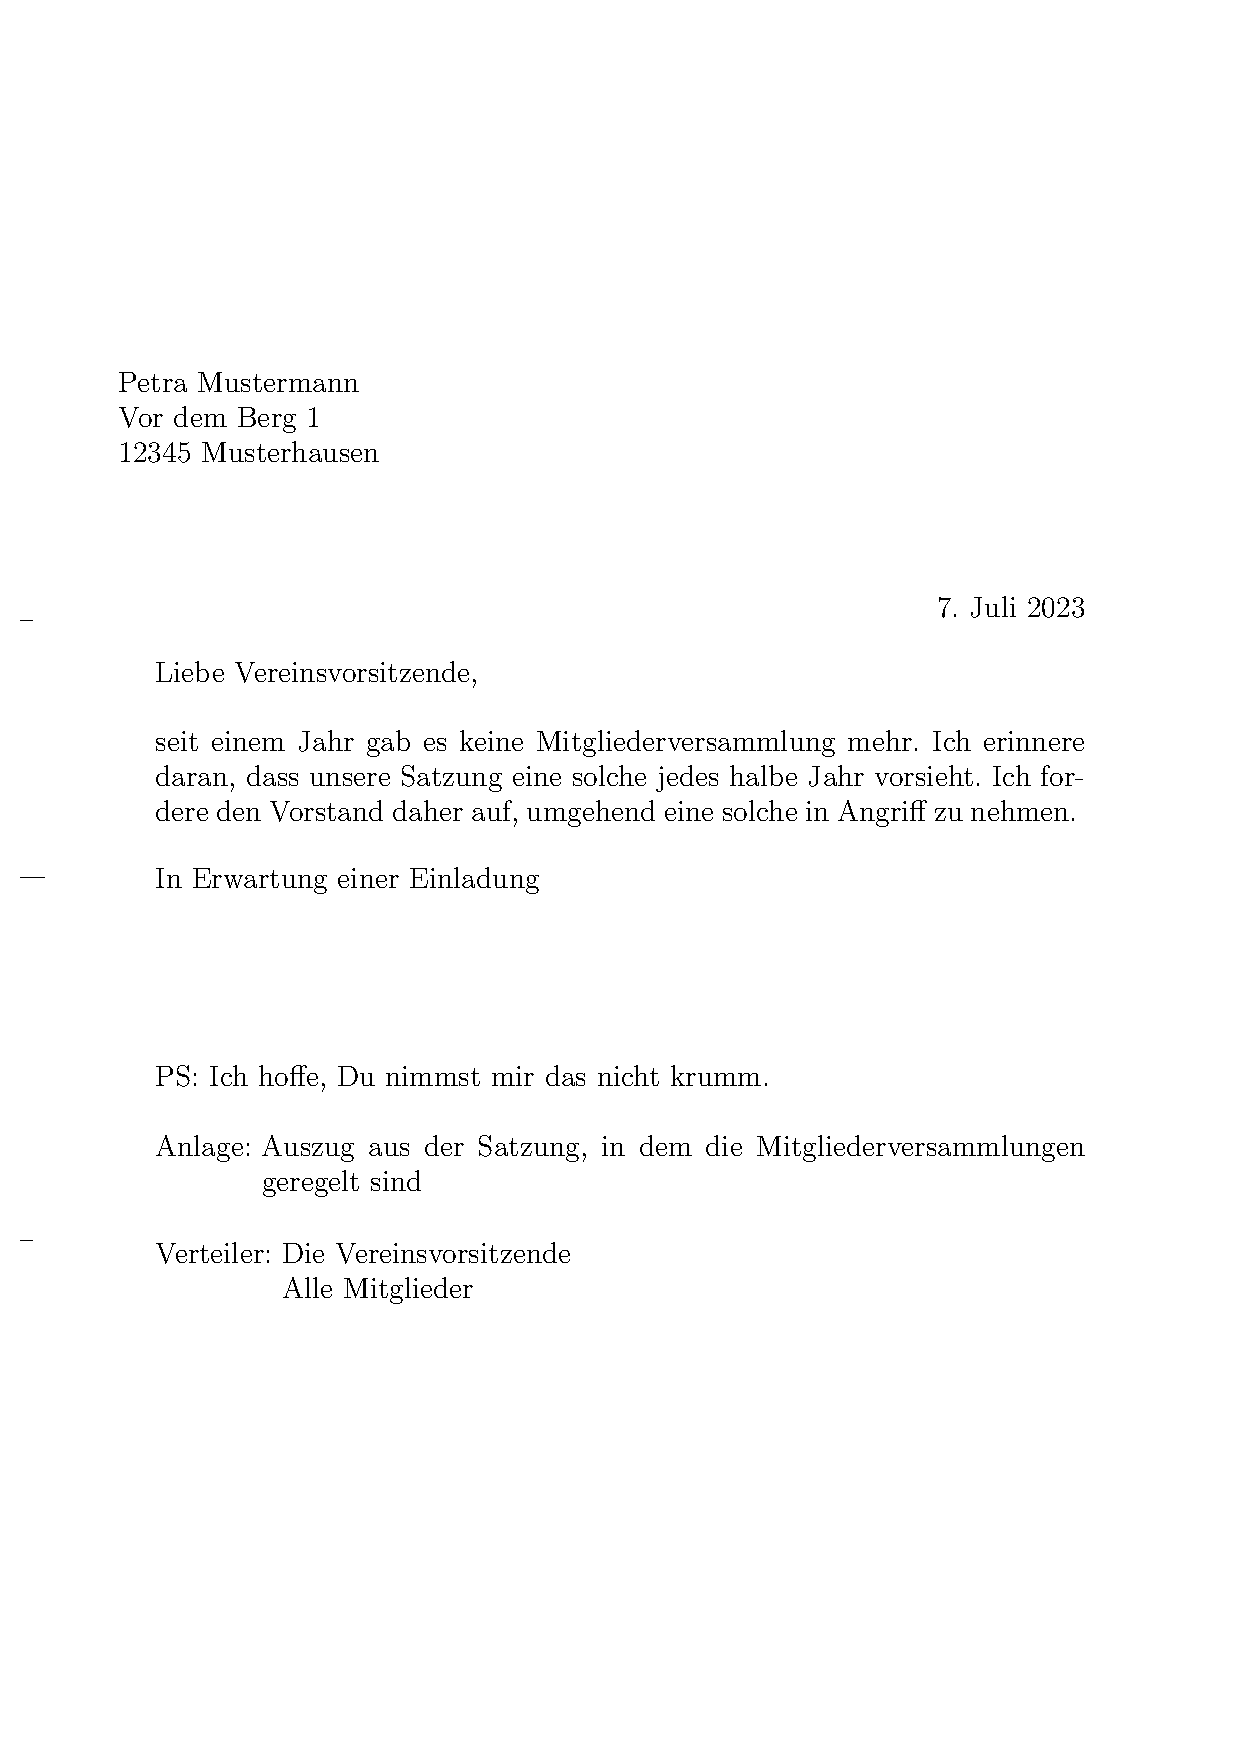
\includegraphics[width=.4\textwidth]{letter-example-05-de}}\quad
      \frame{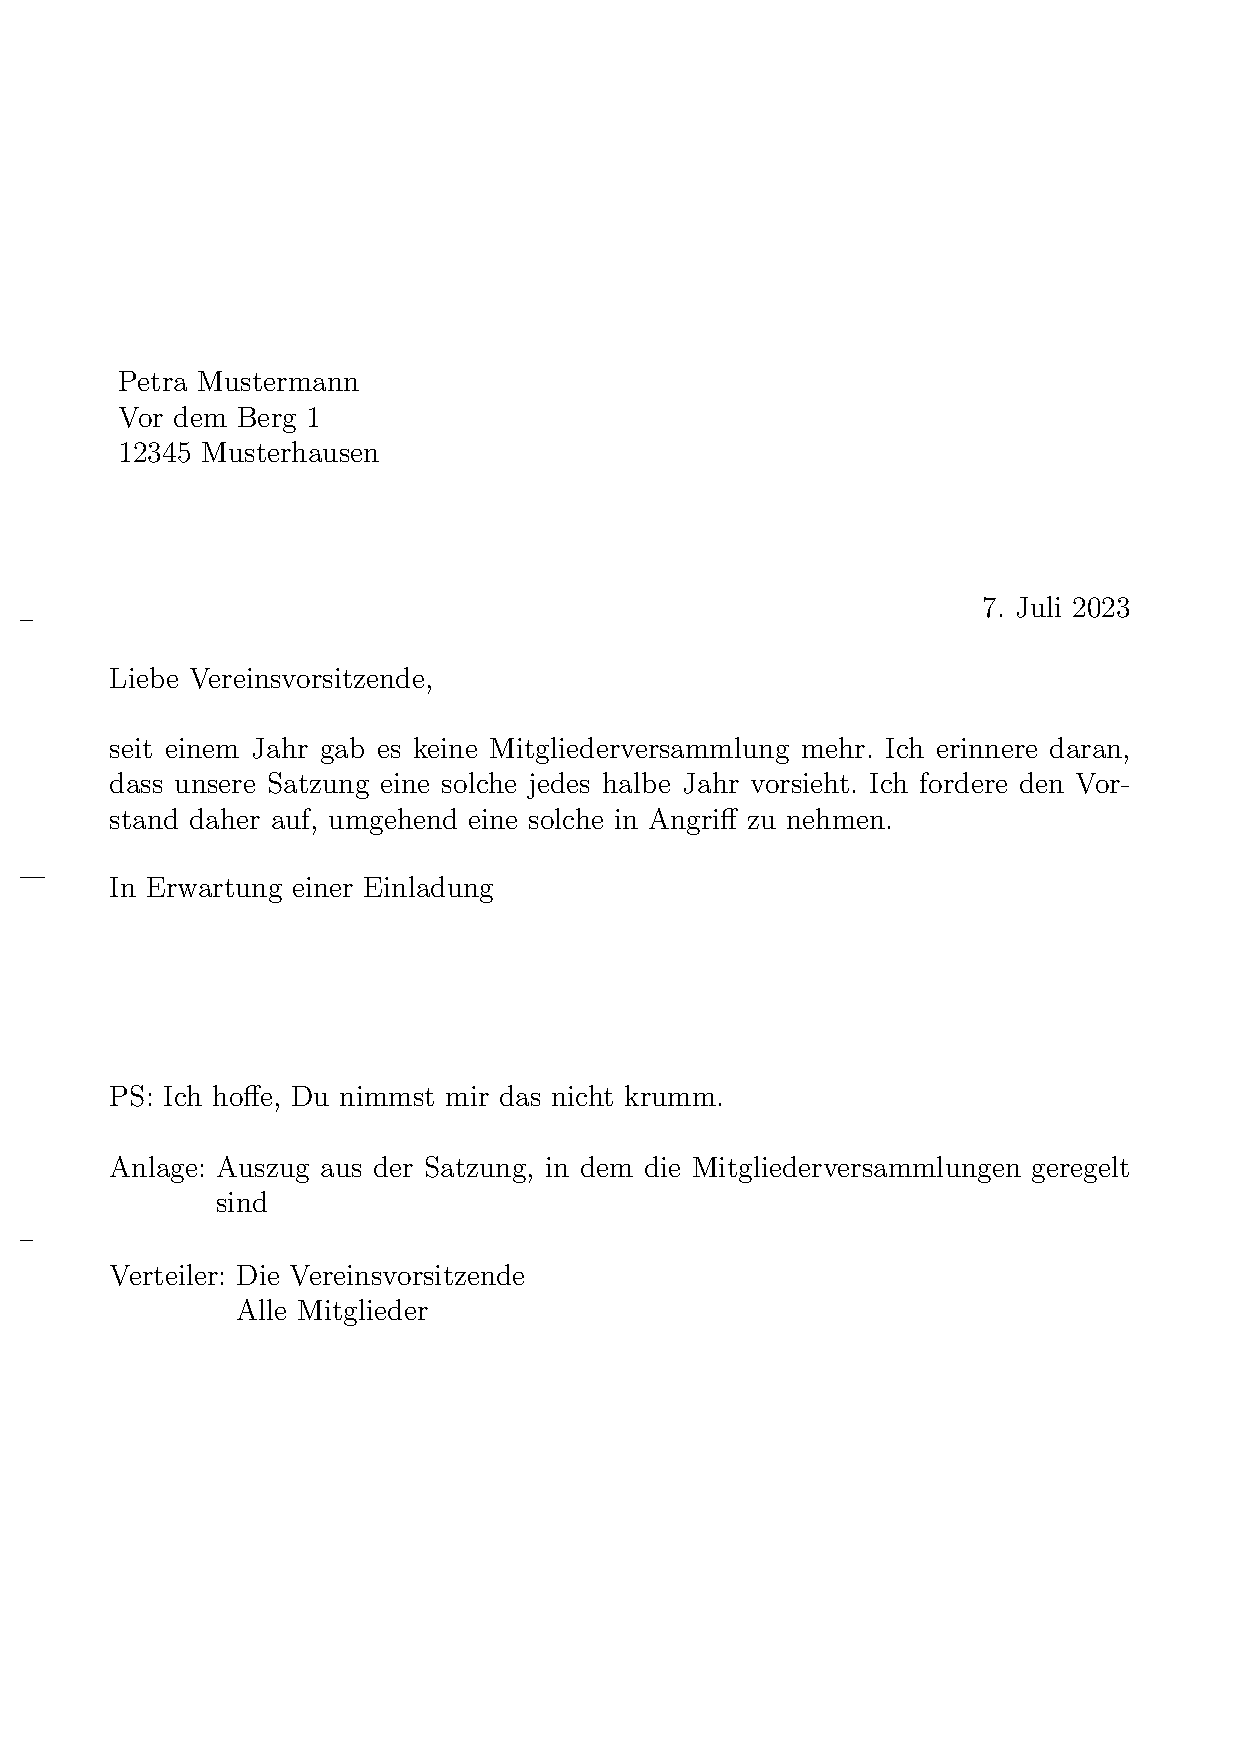
\includegraphics[width=.4\textwidth]{letter-example-06-de}}
%  \end{captionbeside}
      \caption[{Beispiel: Brief mit Anschrift, Anrede, Text,
        Grußfloskel, Postskriptum, Anlagen, Verteiler und ungesund
        großer Schrift}]
      {Ergebnis eines kleinen Briefes mit Anschrift, Anrede, Text,
        Grußfloskel, Postskriptum, Anlagen, Verteiler und ungesund großer
        Schrift (Datum und Faltmarken entstammen den Voreinstellungen für
        DIN-Briefe); links wurde die Schriftgröße als optionales Argument von
        \DescRef{\LabelBase.env.letter} gesetzt, rechts als optionales
        Argument von \DescRef{\LabelBase.cmd.documentclass}}
      \label{fig:scrlttr2.letter-5-6}
    \end{figure}
  \end{Example}%
  \ExampleEndFix
}{%
  \IfThisCommonLabelBase{maincls}{%
    \par
    \phantomsection\label{sec:\ThisCommonLabelBase.fontOptions.end}%
    Voreingestellt ist bei \Class{scrbook}, \Class{scrreprt} und
    \Class{scrartcl} \OptionValue{fontsize}{11pt}.\textnote{\KOMAScript{}
      vs. Standardklassen} Demgegenüber ist bei den Standardklassen
    \Option{10pt} voreingestellt. Dies ist bei einem Wechsel von den
    Standardklassen zu den \KOMAScript-Klassen\iffree{}{ oder bei Verwendung
      von Option \DescRef{maincls-experts.option.emulatestandardclasses}%
      \IndexOption{emulatestandardclasses}} gegebenenfalls zu beachten.% 
  }{}%
}%
\EndIndexGroup
%
\EndIndexGroup

%%% Local Variables: 
%%% mode: latex
%%% TeX-master: "scrguide-de.tex"
%%% coding: utf-8
%%% ispell-local-dictionary: "de_DE"
%%% eval: (flyspell-mode 1)
%%% End: 
